\documentclass[11pt]{article}
\usepackage{graphicx}
\usepackage[bookmarks=true]{hyperref}
\usepackage{bookmark}
\usepackage{hyperref}
\usepackage{csquotes}
\usepackage{float}
\usepackage{wrapfig}
\usepackage{array}
\newcolumntype{L}[1]{>{\raggedright\let\newline\\\arraybackslash\hspace{0pt}}m{#1}}
\newcolumntype{C}[1]{>{\centering\let\newline\\\arraybackslash\hspace{0pt}}m{#1}}
\newcolumntype{R}[1]{>{\raggedleft\let\newline\\\arraybackslash\hspace{0pt}}m{#1}}

\setlength{\parindent}{0pt}

\begin{document}
\begin{titlepage}
\begin{flushright}


\includegraphics[width=380px]{../global/University_of_Pretoria_Logo.png}
\newline
\newline

\textbf {\LARGE Plan for Software Aspects of Certification} \newline

\textbf {\Large (PSAC)} \newline

\centering
\includegraphics[width=100px]{../global/Logo.jpg}

\textbf {\Large Linphone for Android Group Chat (Waterfall)}\newline

\flushright \textbf {\large Version: 1.2}\newline

\centering \textbf {\large Authors:}

\begin{table}[H]
\large
\centering
\begin{tabular}{rl}
	Izak Blom & 13126777 \\
	David Breetzke & 12056503 \\
	Paul Engelke & 13093500 \\
	Prenolan Govender & 13102380 \\
	Jessica Lessev & 13049136 \\
\end{tabular}
\end{table}

Date: \today

\end{flushright}
\end{titlepage}

\setcounter{tocdepth}{3}
\setcounter{secnumdepth}{5}
\tableofcontents

\newpage
\section{User Interface Flow}
The flow chart below illustrates how a user can navigate through the newly added user interfaces and the different paths that the user can follow in order to interact with the newest user interfaces. \\\\
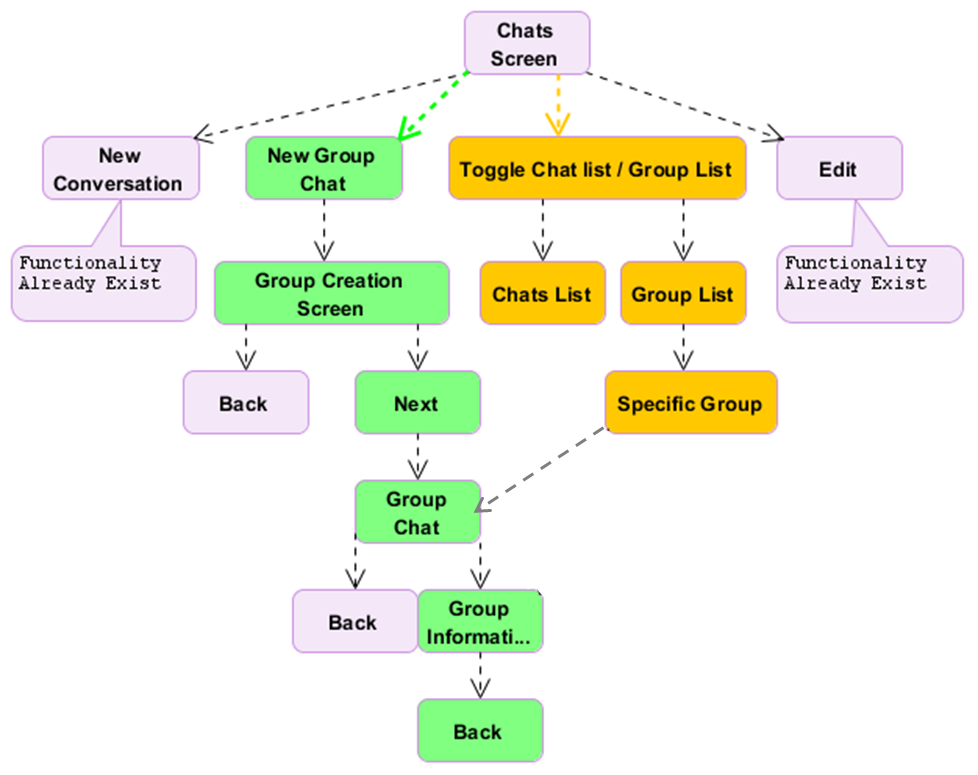
\includegraphics[width=380px]{images/flow.png}

\newpage
\section{User Interfaces}
In this section the newly created user interfaces are listed and shown. The components used to create the user interface are listed along with some implementation details and later on usability comments and motivations are added to certain user interfaces and their components.

\subsection{User Interfaces}

\subsubsection{Chat List User Interface}
The overall function of this interface is to display a list of all the private chats a user currently has open.\\

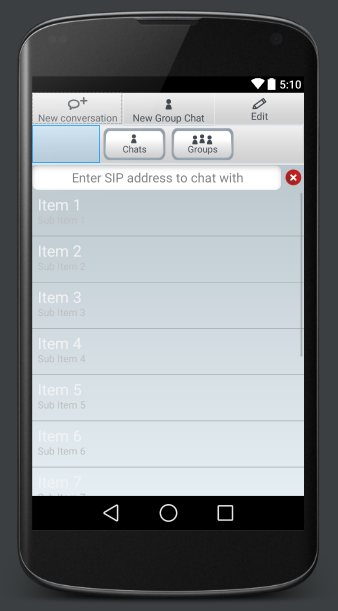
\includegraphics[width=150px]{images/Chatlist.png}
\newpage
\begin{table}[h]
\begin{tabular}{ll}
\textbf{Component}  & \textbf{Function}       
\\ \hline
\multicolumn{1}{|L{5cm}|}{New Conversation Button} & \multicolumn{1}{L{8cm}|}{Provide user the ability to create a new chat with another contact}
\\ \hline
\multicolumn{1}{|L{5cm}|}{New Group Chat Button} & \multicolumn{1}{L{8cm}|}{Provide user the ability to create a new group chat with several other contacts contact}
\\ \hline
\multicolumn{1}{|L{5cm}|}{Edit Button} & \multicolumn{1}{L{8cm}|}{Provide user the ability to remove/delete specific private chats from the chat list}
\\ \hline
\multicolumn{1}{|L{5cm}|}{Chats Toggle} & \multicolumn{1}{L{8cm}|}{Provide user the ability to switch between their list of private chats currently open and their list of group chats they are currently involved in. Clicking on the "Chats" toggle will display the list of private chats.}
\\ \hline
\multicolumn{1}{|L{5cm}|}{Groups Toggle} & \multicolumn{1}{L{8cm}|}{Provide user the ability to switch between their list of private chats currently open and their list of group chats they are currently involved in. Clicking on the "Groups" toggle will display the list of group chats.}
\\ \hline
\multicolumn{1}{|L{5cm}|}{Text Edit to enter SIP address} & \multicolumn{1}{L{8cm}|}{Provide user the ability to perform a "quick search" in their list of private chats to find a specific chat.}
\\ \hline
\multicolumn{1}{|L{5cm}|}{Red "X" next to Text Edit} & \multicolumn{1}{L{8cm}|}{Allows the user to clear the text edit when desired.}
\\ \hline
\multicolumn{1}{|L{5cm}|}{List} & \multicolumn{1}{L{8cm}|}{This is the actual list of private chats. Clicking on a chat from the list will open the corresponding chat -> chat user interface}
\\ \hline

\end{tabular}
\end{table}
\end{document}
